\textbf{Beispiel 1} \\ \\
a) \\ \\
Bei diesem Messversuch treten Haftreibung
\[
	f_H = \mu_Hmg
\]
trockene Gleitreibung
\[
	f_C = \mu_C m g \, \text{sign}\dot{x}
\]
und viskose Reibung
\[
	f_r = \mu_V \Delta v
\]
auf.
Im folgenden werden diese drei Fälle unterschieden
\[
	f_e = \begin{cases}
		f_H & \text{für} \, \dot{x} = 0 \\
		f_C + f_r & \text{sonst}
	\end{cases}
\]
b) \\ \\
Reibparameter:
\begin{align*}
	\mu_H &= \frac{f_H}{mg} = \frac{0.1 N}{1kgms^{-2}} = 0.1 \\
	\mu_C &= \frac{f_C}{mg} = \frac{0.1 N}{1kgms^{-2}} = 0.1 \\
	\mu_V &= \frac{f_r}{\Delta v} = \frac{0.1N}{1ms^{-1}} = 0.1 Nsm^{-1}
\end{align*}
c) \\ \\
\begin{figure}[h]
	\centering
	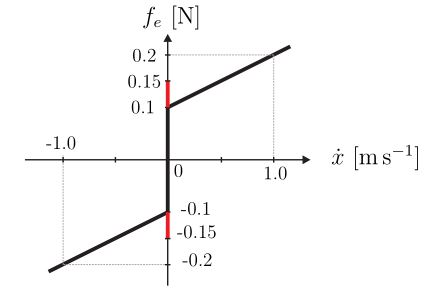
\includegraphics[width=8cm]{tikz/11_03_2016_1c}
\end{figure}